%% This is an example first chapter.  You should put chapter/appendix that you
%% write into a separate file, and add a line \include{yourfilename} to
%% main.tex, where `yourfilename.tex' is the name of the chapter/appendix file.
%% You can process specific files by typing their names in at the 
%% \files=
%% prompt when you run the file main.tex through LaTeX.
\chapter{Design Options}
\label{ch:design}

GPU architecture is significantly different than that of a CPU, and thus a high performance PIC code on a GPU is going to look a lot different from its CPU equivalent. Memory access patterns, cache behavior, thread communication, and thread workload all have significant impacts on the performance of GPU codes. This means that porting an existing PIC code to the GPU is by no means straightforward, the data structures and algorithms will likely be different from the original serial code. 

Performance is just one facet of the code design, maintaining separate CPU and GPU versions of the same code presents additional problems. Programmers tend to be lazy in that the fewer lines of code that they have to write, the better. If a new feature is desired, then two different implementations of that feature must be written and debugged. From the lazy programmers perspective this is to be avoided as much as possible. Therefore, it is very important that the GPU version of the code utilize as much of the CPU code as possible. This means that interoperability between the CPU and GPU code must be both efficient and fast. 

Performance and maintenance are the two key issues that were considered when designing sceptic3Dgpu. Some of these issues have been investigated previously, although the amount of research in this area is still very small. To make matters worse, the specific techniques used are rapidly evolving with every new generation of graphics card. It is unlikely that the pace of GPU hardware evolution will slow in the near future. Spending large amounts of time optimizing algorithms for the current generation of hardware is inadvisable, and therefore the design of the code should focus on utilizing techniques that emphasize the underlying principles of GPU design or utilize library functions that will be optimized for each generation of hardware. 

The goal of this chapter is to outline various design options for implementing the various steps of the PIC algorithm on the GPU and explore the pros and cons of each option. Solutions used by other researchers will be outlined and evaluated based on their applicability to sceptic3D and their applicability to PIC codes in general. To accelerate these evaluations a simple 3D sandbox PIC code was implemented on the GPU in addition to several other basic comparison codes. 

%%%%%%%%%%%
%This means that separate CPU and GPU versions of the code must be maintained depending on the features desired for each architecture. Maintaining two separate versions of a code and as such it is important that the focus of GPU PIC code development be focused on steps of the PIC algorithm that are the most computationally intensive. Steps should be taken during the development to 


%For a serial or even MPI PIC implementations there is enough memory that each thread can have a separate copy of the grid and only need to talk to one another after chugging through a massive list of particles. In these cases the communications costs are negligible compared to the computations performed by each thread. On the GPU the situation is a lot different. Instead of a few threads doing lots of work you have a lot of threads doing little work. 
%%%%%%%%%%%
%%%%%%%%%%%%%%%%%%%%%%%%%%%%%%%%%%%%
	\section{GPUPIC Sandbox and the big questions}
%%%%%%%%%%%%%%%%%%%%%%%%%%%%%%%%%%%%
The first step in the development of sceptic3Dgpu was to create a very simple, generalized pic code that performed the major steps of the PIC algorithm and implement it in CUDA. This simple code, we'll call it GPUPIC\_testbed is designed without making any assumptions about the physics of the system. GPUPIC\_testbed operates in Cartesian coordinates with periodic boundary conditions. We do not really care too much about the field solve since in the serial version it takes a very small amount of time compared to the particle advance and charge assign steps. By recognizing the low priority of the field solve we really only need to characterize the performance of the following 5 steps:


\begin{enumerate}\itemsep0pt \parskip0pt \parsep0pt
\item Read the particle data
\item Read the Potential data for that particle
\item Move the particle
\item Write the new particle data back to the particle list
\item Interpolate Charge to Mesh
\item Goto 1
\end{enumerate}



The first implementation of this code was very naive. The only real difference from a serial version was the density array update, which used atomic updates on global memory in order to prevent memory collisions between multiple threads. Other than that the code boiled down to unrolling the loop over all of the particles into one particle per thread. The runtime breakdown of this code for a $32^3$ grid and 4.2 million particles is shown in table \ref{tab:GPUPIC_basetime}.

\begin{center}
\begin{table}
\begin{tabular}{| p{4.0cm} | p{3.5cm} |}
\hline
Component & Runtime (ms) \\ \hline
Particle data read, move, and write & 375 \\ \hline
Potential Grid Read & 467 \\ \hline
Charge Assign & 1.143e4  \\ \hline
Total & 1.227e4  \\ \hline
\end{tabular}
\caption{Total Execution times for 100 iterations of the key steps of the move kernel at three different optimizations.}
\label{tab:GPUPIC_basetime} 
\end{table}
\end{center}

As you can see, the particle move and the potential read are very similar, but the charge assign is very slow. Determining how we can better adapt the charge assign to the GPU is our first major challenge. Several ways of dealling with the issue of the charge assign will be discussed in the following section. Some of the other issues that will be discussed in this chapter are:

\begin{itemize}\itemsep0pt \parskip0pt \parsep0pt
\item Particle Data Structure: Is it better to use an Array of structures, like the fortran code, or a Structure of Arrays?
\item How do we handle divergent processes in the advancing routine, such as losses, reinjections, and collisions?
\item At what point does the field solve become a dominant cost?
\item Are there any new issues that arise from solutions to the other issues?
\end{itemize}

%%%%%%%%%%%%%%%%%%%%%%%%%%%%%%%%%%%%
	\section{Charge Assign}
%%%%%%%%%%%%%%%%%%%%%%%%%%%%%%%%%%%%

There are two different ways to approach the charge assign, one in which information is ``pulled" from the particles by the vertices, and one in which data is ``pushed" by the particles to the vertices. Let G represent a grid of domain D of dimension d comprised of all vertices $v_s  \in \mathrm{D}$. We can define some distribution function $f(v_s)$ at each of the vertices which is the sum of some function $\mathrm{K}(v_s,p_i)$, where $p_i$ is the position of particle $i$. Given these definitions the algorithms for the particle pull and particle push method are algorithms \ref{alg:particle_pull} and \ref{alg:particle_push} respectively. 

\begin{algorithm}
	\begin{algorithmic}
		\STATE // Loop over the verticies first
		\FORALL{$\mathrm{vertex} \: v_s \in G$}
			\STATE find $\mathcal{P}(v_s)$
			\STATE $\mathrm{f}(v_s) \leftarrow 0$
			\FORALL{$p_i \in \mathcal{P}(v_s)$}
			\STATE $\mathrm{f}(v_s) \leftarrow \mathrm(f)(v_s) + \mathrm{K}(v_s,p_i)$
			\ENDFOR
		\ENDFOR
	\end{algorithmic}
	\caption{Particle Pull Method of charge deposition. From Stantchev et al. \cite{Stantchev2008}}
	\label{alg:particle_pull}
\end{algorithm}

\begin{algorithm}
	\begin{algorithmic}
		\STATE // Loop over the verticies first
		\FORALL{$\mathrm{vertex} \: v_s \in G$}
			\STATE $\mathrm{f}(v_s) \leftarrow 0$
		\ENDFOR
		\FORALL{$\mathrm{particle} \: p_i \in \mathrm{D}$}
			\STATE find $\mathcal{V}(p_i)$
			\FORALL{$v_s \in \mathcal{V}(p_i)$}
				\STATE $\mathrm{f}(v_s) \leftarrow \mathrm(f)(v_s) + \mathrm{K}(v_s,p_i)$
			\ENDFOR
		\ENDFOR
	\end{algorithmic}
	\caption{Particle Push Method of charge deposition. From Stantchev et al. \cite{Stantchev2008}}
	\label{alg:particle_push}
\end{algorithm}

As pointed out by \cite{Stantchev2008} each method has its advantages and disadvantages. 


Looking back at table \ref{tab:GPUPIC_basetime} we notice that the charge assign step constitutes about 93\% of the total runtime.  Unfortunately this poor performance is a result of serialization caused by the atomic updates. Additionaly, since the grid is far too large to fit in shared memory these updates must be performed on global memory, which has much higher latency and lower bandwidth. When a thread attempts to update a value in memory and finds that it is locked it must then repeat the process until it succeeds. Every failed update represents an additional slow global memory access that is essentially wasted. 

\begin{figure}
\begin{center}
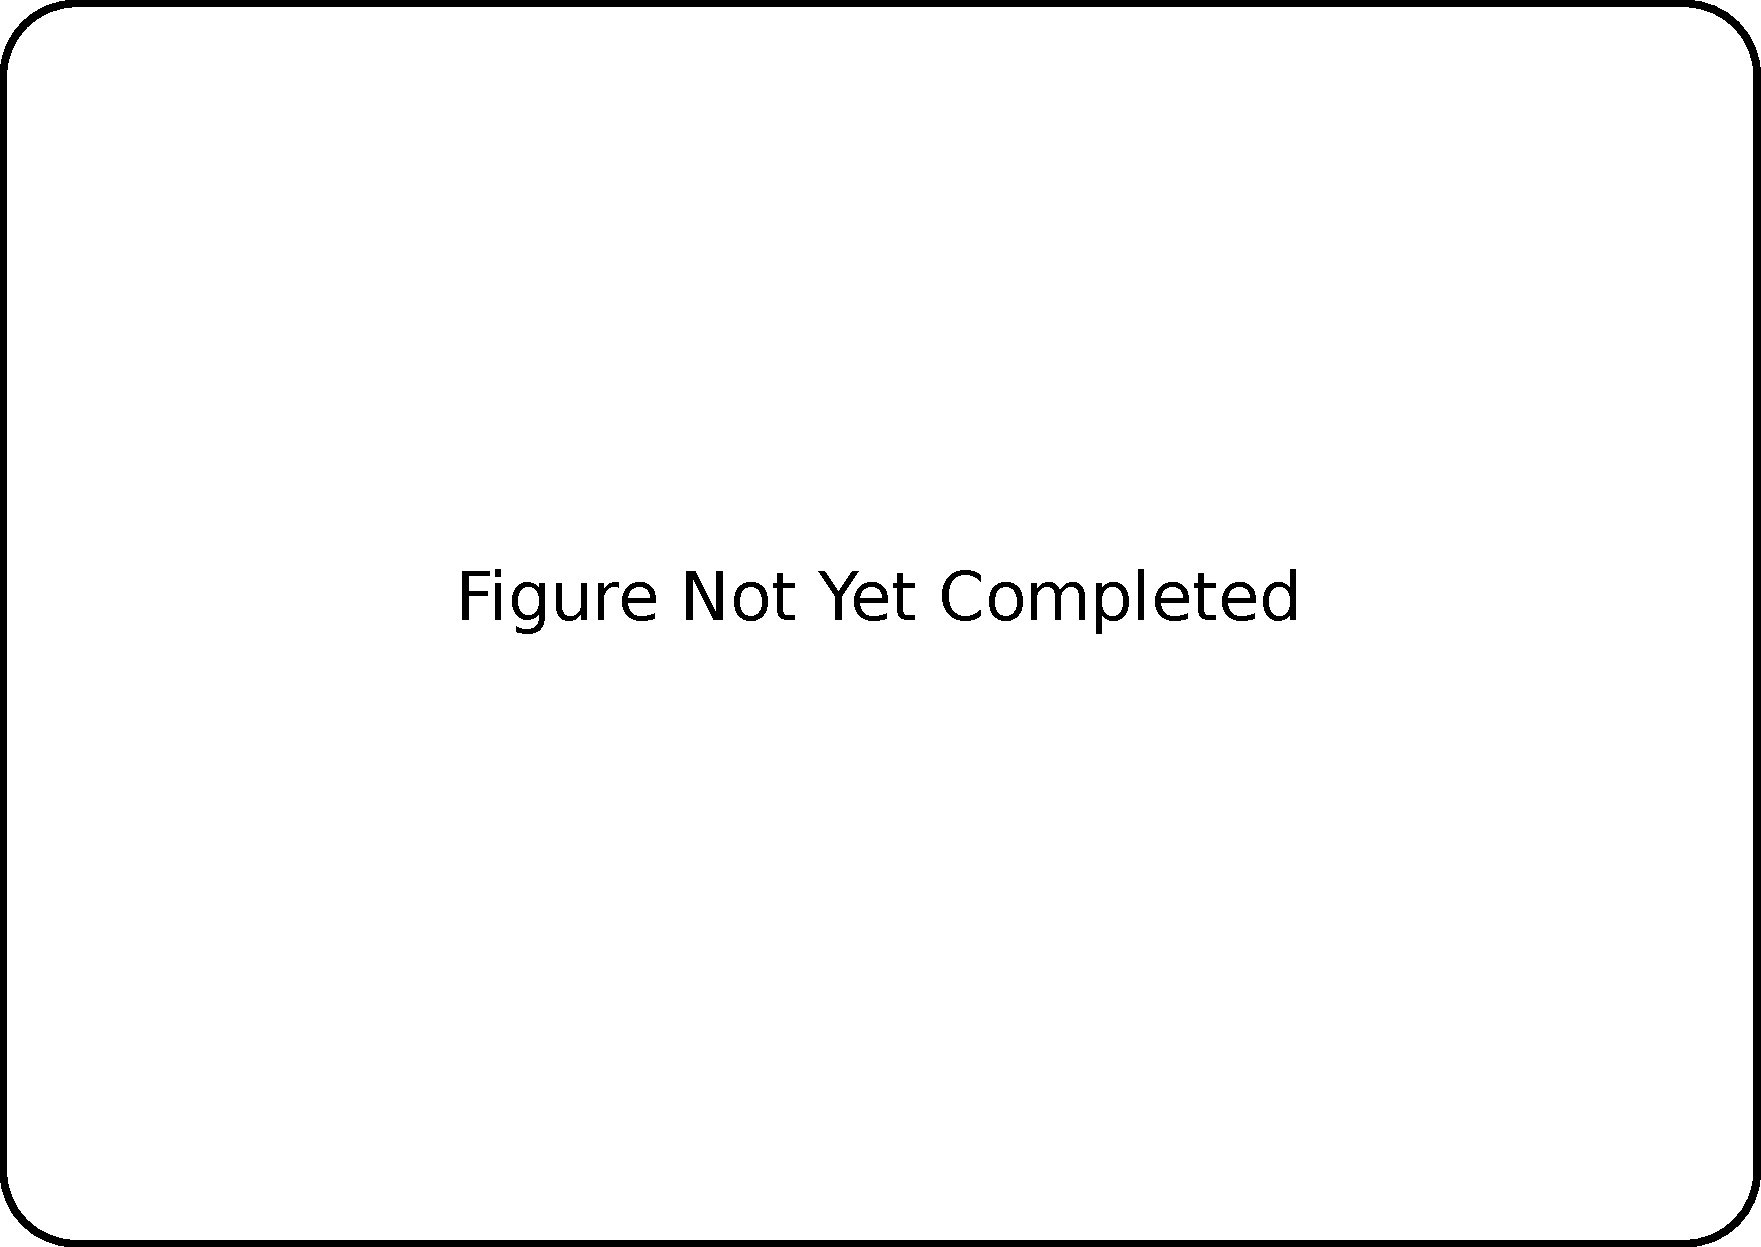
\includegraphics[width=4in]{introduction/not_finished.pdf}
\end{center}
\caption{Atomic Memory collisions}
\label{fig:pic_flowchart_parallel}
\end{figure}

The technique applied for MPI codes is parallel reduction. Each thread deals with a subset of the particle list and tallies up the contributions of that list to some array in memory private to a single thread. Once every thread has recorded the contributions from their subset of the particle list a parallel reduction is performed in order to quickly sum up the contributions from all threads. The problem with directly applying this solution to the GPU is that when a thread reads in a particle the thread must be able to account for every possible location that the particle can contribute to. With a completely random particle list any given particle can contribute to any element of the grid. However, say a thread knows that every particle that it reads in will only contribute to one element of the grid. This thread now only has to keep track of a single value, since it knows that every particle it sees will only contribute to this value. When it comes time for all of the threads to contribute to the final result each thread provides the full answer for a single element. This method significantly reduces the memory requirements of each thread but imposes the constraint that a thread is given only particles that exist within its domain. We will worry about this additional constraint later. 

\begin{figure}
\begin{center}
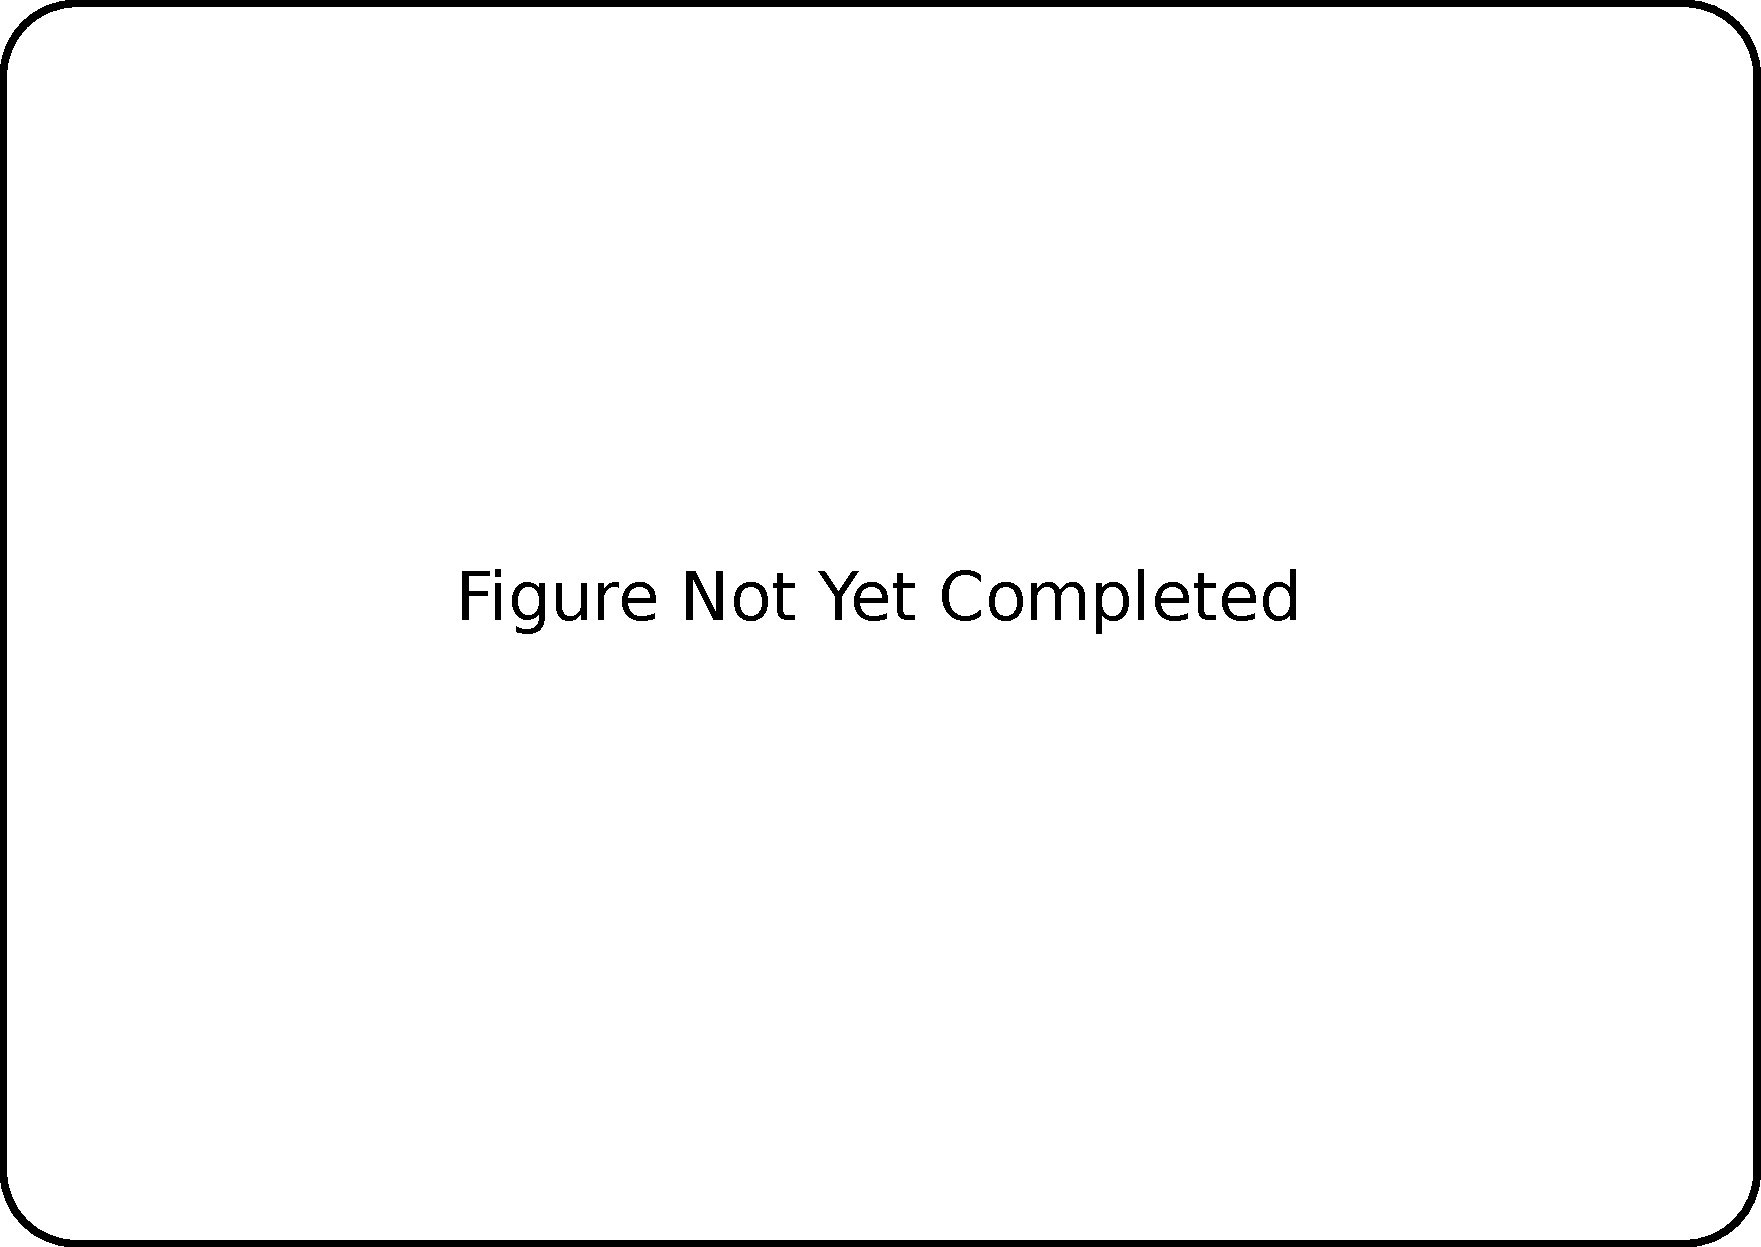
\includegraphics[width=4in]{introduction/not_finished.pdf}
\end{center}
\caption{One thread per cell}
\label{fig:pic_flowchart_parallel}
\end{figure}

Now consider this, the MPI code works well for a few randomly ordered sets of many particles, or objects, manipulated by a small number of threads. The decomposition technique works for a small number of organized sets of a few objects manipulated a large number of threads. If we think of threads operating on small groups of particles as objects and we replace every instance of `objects' with `threads' in the previous two sentences we end up with an interesting situation. Apply the MPI technique to a few randomly ordered sets of many threads each operating on a small number of particles. Essentially if we want to run really large particle lists we can divide up the list amongst several nodes. Each node uses many threads to process a small ordered subset of this list and contribute to the full array. Once every node has completed its own tally the standard MPI technique is used to gather the tallies of all the nodes. This is an excellent example of multi-grained parallelism. The level consisting of multiple nodes is coarse parallelism while the node level is a finer level of parallelism.   

\begin{figure}
\begin{center}
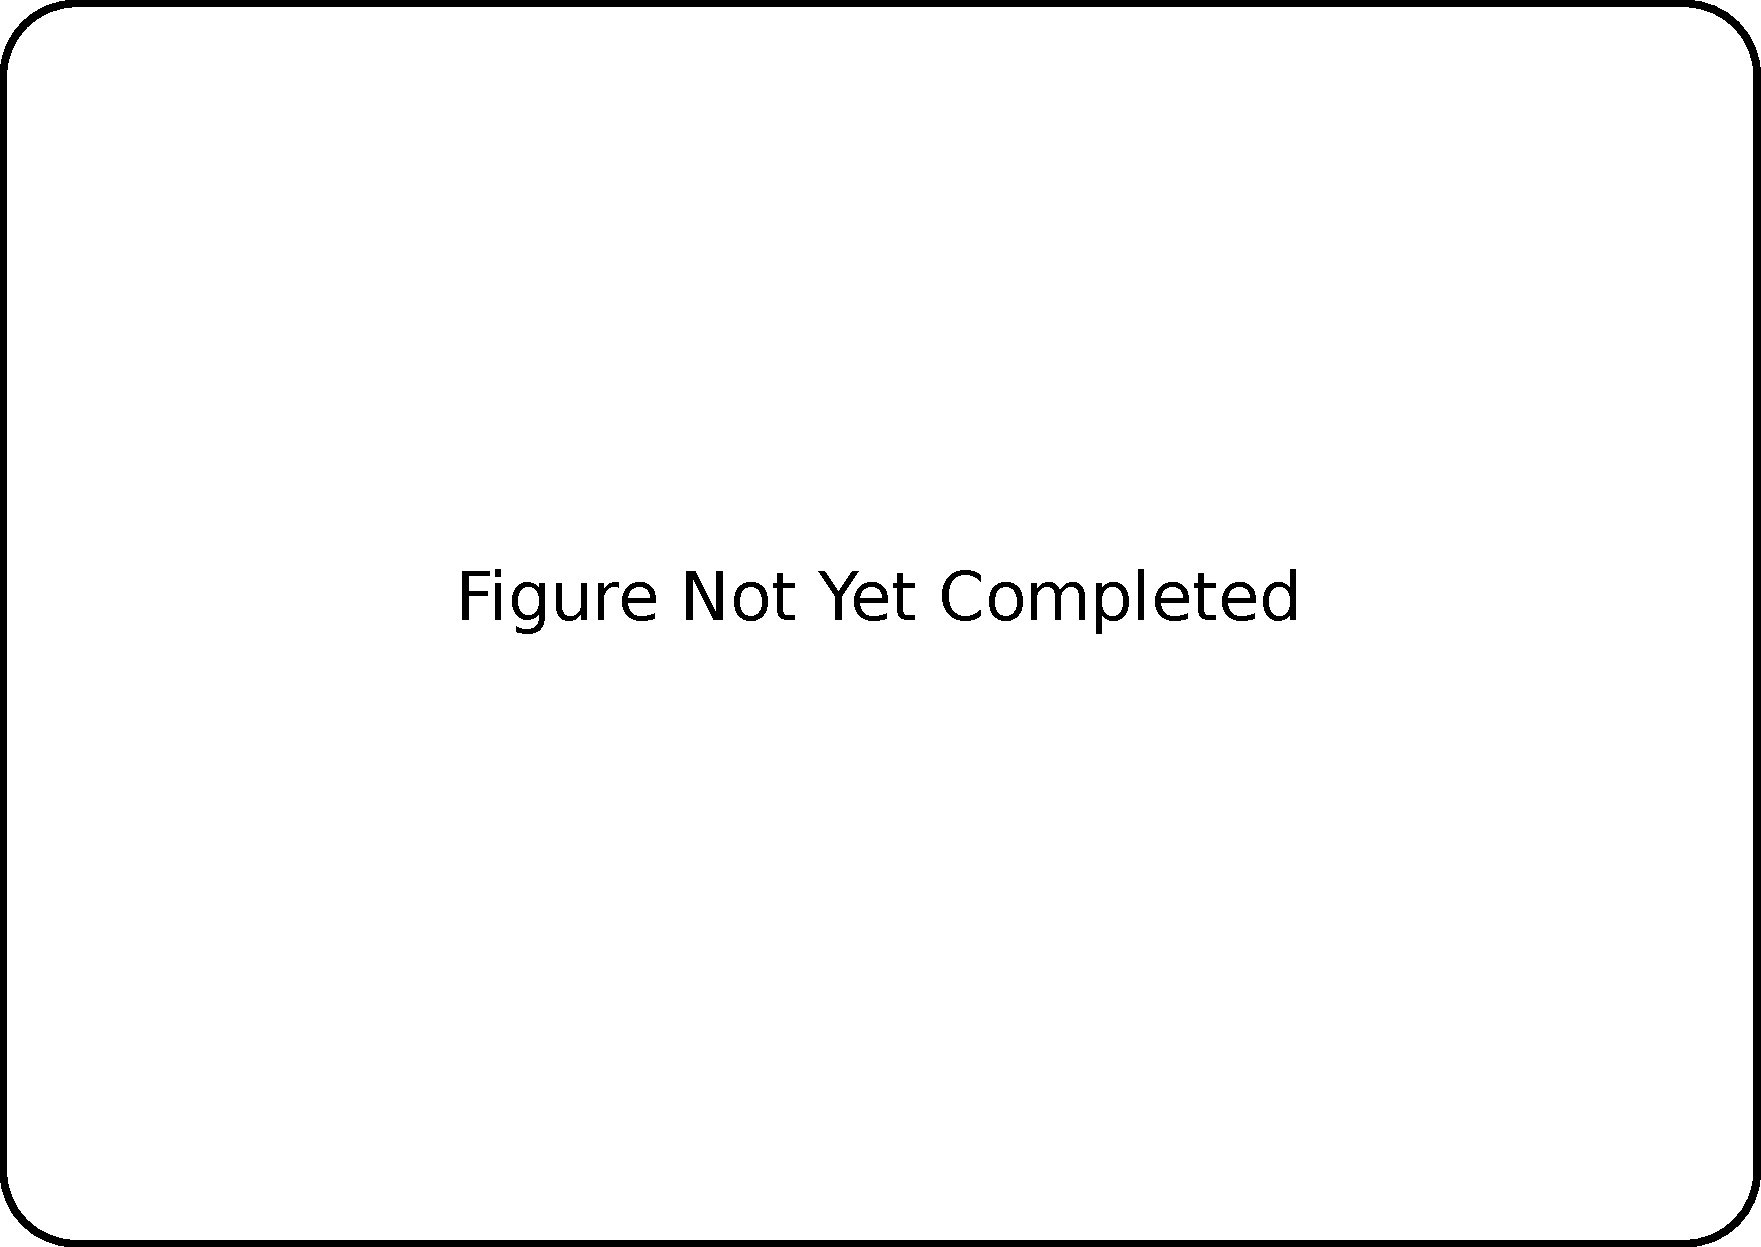
\includegraphics[width=4in]{introduction/not_finished.pdf}
\end{center}
\caption{MPI and One thread per cell}
\label{fig:pic_flowchart_parallel}
\end{figure}

We can take this methodology even further on the GPU by recognizing that we can parallelize the single element summations using reductions. Taking this to the limit of one thread per particle on the GPU we end up with each thread block, or several blocks, is responsible for a subset of the particle list. All of the particles in the block's list will contribute to the same element. The threads within each block read in their particles contribution to that element into shared memory. With all of the data in shared memory a very fast parallel reduction can be performed. 

\begin{figure}
\begin{center}
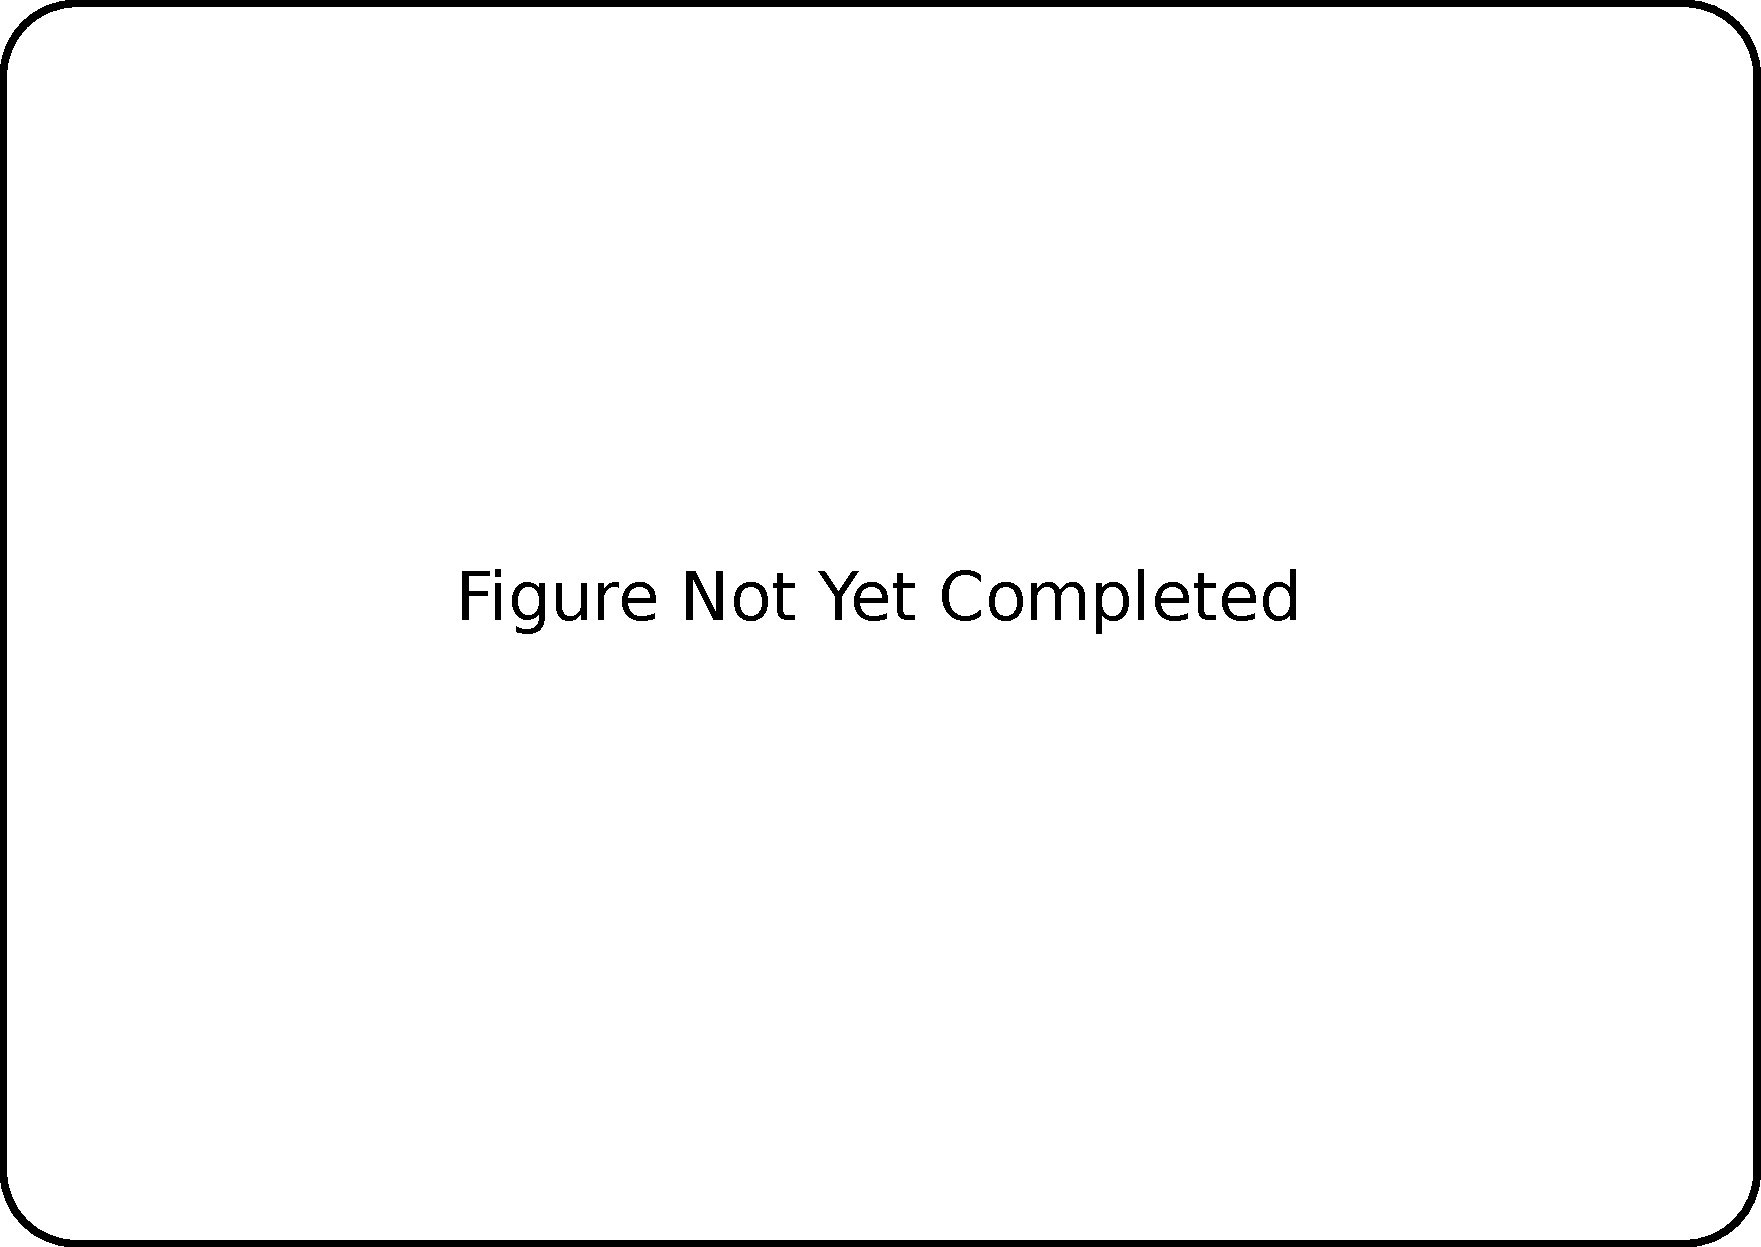
\includegraphics[width=4in]{introduction/not_finished.pdf}
\end{center}
\caption{Three levels of parallelism for the charge assign}
\label{fig:pic_flowchart_parallel}
\end{figure}

We implemented this technique in the sandbox PIC code and compared the runtime of the reduction method to the atomic version. The results of this comparison can be seen in table \ref{tab:GPUPIC_comparison}.

\noindent \begin{table}
\begin{tabular}{| p{4.0cm} | p{3.5cm} | p{3.5cm} |}
\hline
Component & Atomic-Updates (ms) & Sorted+Reduction (ms) \\ \hline
Particle data read, move, and write & 375 & 468 \\ \hline
Potential Grid Read & 467 & 285 \\ \hline
Charge Assign & 1.143e4 & 542 \\ \hline
Particle List Sort & 0 & 2.305e3 \\ \hline
Total & 1.227e4 & 3600 \\ \hline
\end{tabular}
\caption{Total Execution times for 100 iterations of the key steps of the move kernel at two different optimizations.}
\label{tab:GPUPIC_comparison}
\end{table}
As you can see from the table, the charge assign is on the order of 20x faster using the reduction technique, although this speedup is somewhat offset by the sorting requirement. Sorting the particles also benefits reading the potential during the advancing step. This speedup is a result of increased cache hits due to all threads within the same thread block accessing the same addresses in the potential array. 

Although we have successfully reduced the cost of the charge assign we have introduced an additional cost of a sorting step. In the case of the sandbox code the sort step accounts for roughly 70\% of the runtime. Fortunately several other projects have figured out that there are ways reduce the sorting costs while maintaining some of the performance achieved by utilizing a sorted particle list. 

 
		\subsection{Other Codes}
There are several papers which point out that sorting by cell at every time step is not entirely necessary. It is possible to minimize the sorting requirement by expanding the sorting bins to include multiple cells, or rather, by dividing the simulation space into slabs composed of multiple cells. The advantage to this technique is sorting is only required between slabs, but not within the slabs.\cite{Abreu2011} 

This slab method, as described by Abreu et al, is used on a one thread per slab basis. One thread for each slab loops over all of the particles that belong to that slab, contributing to an array that is the same size as the slab. Once a thread completes its particle loop it writes the portion of the array that it is responsible for to the main array, using atomic operations for guard cells.\cite{Abreu2011} 

A similar approach is employed by Stantchev et al \cite{Stantchev2008}. 





%%%%%%%%%%%%%%%%%%%%%%%%%%%%%%%%%%%%
	\section{Particle List Sort}
%%%%%%%%%%%%%%%%%%%%%%%%%%%%%%%%%%%%
		\subsection{Costs and Benefits}
		\subsection{Other Codes}
		*Stantchev Particle Binning
		*Kong Particle Passing
		*Linked Particle List
		\subsection{In house tests}

%%%%%%%%%%%%%%%%%%%%%%%%%%%%%%%%%%%%
	\section{Particle List Structure}
%%%%%%%%%%%%%%%%%%%%%%%%%%%%%%%%%%%%
	
		\subsection{Other Codes}
		\subsection{In house tests}
\noindent \begin{table}[h]
\begin{tabular}{| p{4.0cm} | p{3.5cm} | p{2.5cm} | p{4.0cm} |}
\hline
Component & SoA (ms) & AoS (ms) & Speedup (SoA vs AoS) \\ \hline
Particle data read, move, and write & 758 & 955 & 1.26x \\ \hline
Count Particles & 32.7 & 109 & 3.35x \\ \hline
Data Reorder & 346 & 480 & 1.38x \\ \hline
Total CPU run time & 2491 & 3284 & 1.31x \\ \hline
\end{tabular}
\caption{Execution times of main steps for Array of Structures and Structure of Arrays. Count Particles and Data Reorder are steps used for a sorted particle list. Count Particles counts the number of particles in each sub-domain. Data Reorder reorders the particle list data after the binindex / particle ID pair have been sorted by the radix sort.}
\label{tab:struct_compare} 
\end{table}

	\section{Particle Advancing}
		\subsection{Assumptions}
		\subsection{Other Codes}
		\subsection{Reinjections and Diagnostics}

	\section{Poisson Solve}
		\subsection{Desired Performance}
		\subsection{Performance vs Implementation Difficulty}

	\section{Grid Dimension Constraints and Handling}
